\documentclass{article}
\usepackage[T1]{fontenc}
%\usepackage[top=1in,left=.75in, right=.75in, bottom=1in]{geometry}
\usepackage{cprotect}
\usepackage{float}
\usepackage{inconsolata}
\usepackage{listings}
\usepackage{microtype}
\usepackage{relsize}
%\usepackage[skins]{tcolorbox}
\usepackage{tikz}
\usepackage{xcolor}
\usepackage{hyperref} % use hyperref package last

\usetikzlibrary{calc,shapes.multipart,chains,arrows}
\tikzset{
  list/.style={ % image of a singly-linked list node
    very thick, rectangle split,
    rectangle split parts=2, draw,
    rectangle split horizontal, minimum size=18pt,
    inner sep=4pt, text=black,
    rectangle split part fill={red!20, blue!20}
  },
  dlist/.style={  % image of a doubly-linked list node
    very thick, rectangle split,
    rectangle split parts=3, draw,
    rectangle split horizontal, minimum size=18pt,
    inner sep=5pt, text=black,
    rectangle split part fill={blue!20, red!20, blue!20}
  },
  dummy/.style={  % Image of a dummy node
    draw,rectangle,minimum size=18pt, fill=orange!80,
    inner sep=0pt, text=black,
    path picture = {
      \draw[black]
      (path picture bounding box.north west) --
      (path picture bounding box.south east)
      (path picture bounding box.south west) --
      (path picture bounding box.north east);
    }
  },
  endlist/.style={
    draw, rectangle, minimum height=18pt, minimum width=30pt, gray, thick, dashed
  }
}

\hypersetup{
  colorlinks=true,
  linkcolor=blue,
  urlcolor=blue,
  pdftitle={An Introduction to Linked Lists},
  pdfauthor={Jeff Bienstadt},
  pdfsubject={Linked List},
  pdfkeywords={linked list, computing, data structures, C, C++}
}

\lstset{
  basicstyle        = \small\ttfamily,
  keywordstyle      = \color{blue}\textbf,
  commentstyle      = \color{gray}\rmfamily\itshape,
  columns           = fullflexible,
  numbers           = left,
  numberstyle       = \scriptsize\sffamily\color{gray},
  showstringspaces  = false,
  keepspaces        = true
}

\lstnewenvironment{algorithm}[1][] %defines the algorithm listing environment
{
    \lstset{
        mathescape=true,
        frame=tB,
        numbers=left,
        numberstyle=\tiny,
        basicstyle=\small\em,
        keywordstyle=\color{black}\bfseries,
        keywords={return, if, else, foreach, do, while, begin, end, procedure},
        numbers=left,
        xleftmargin=.04\textwidth,
        #1
    }
}{}
\lstnewenvironment{lstc}[1][firstnumber=last]{\lstset{language=C,#1}}{}
\lstnewenvironment{lstcpp}[1][firstnumber=last]{\lstset{language=[11]C++,name=cpp,#1}}{}

\newcommand{\Cpp}{\mbox{C\kern-.1em\raisebox{.35ex}{\smaller{\smaller{+\kern-0.05em+}}}}}

\begin{document}
  \title{An Introduction to Linked Lists}
  \author{Jeff Bienstadt}
  \date{December 15, 2021}
  \maketitle
  \begin{abstract}
    This article presents the linked list data structure. It describes the layout of the linked list and the operations that can be performed with its use. Finally, it presents annotated source code for implementations in the C and \Cpp\ languages. The full source code, in both languages, including code to demonstrate the usage of linked lists in applications, is available for download from GitHub\footnote{\url{https://github.com/jeffbi/data-structures/tree/master/LinkedList/C}}\footnote{\url{https://github.com/jeffbi/data-structures/tree/master/LinkedList/C++}}.
  \end{abstract}
  \part{Description}\label{part:description}
  The linked list is a linear data structure that consists of a series of \emph{nodes} that contain the data and which are \emph{linked} together. The data portion of a node may contain any type of data desired. This article will use simple integer values for node data.

  The first node in the linked list is the \emph{head} node. An implementation will generally keep a pointer or reference to the head node as a way of keeping track of the linked list itself. A linked list with no head node is empty. The last node in the linked list is the \emph{tail} node. Some implementations also keep track of the tail node, but it is not required.

  Nodes in a linked list are not required to be contiguous in memory, and they are unlikely to be. Because nodes are linked rather than each residing in a specific location as in an array, a linked list may ``grow'' or ``shrink'' to any size required, without the need to move any surrounding nodes. As a result inserting a new node into the list is fast and efficient. However, locating a given node is comparatively slow as the linked list does not provide for quick random access. Instead the list must be traversed node by node until either the desired node is found or until a terminating node is reached.

  There are two types of linked lists: the singly-linked list and the doubly-linked list. This article will present both of these types.
  \section{Singly linked lists}
  A singly-linked list uses nodes that contain the node's data and contain a single pointer to the next node in the list. Singly-linked lists may be traversed in only one direction, toward the list's tail.

  Figure~\ref{fig:singlelinkedlist} is a conceptual view of what a singly-linked list might look like.
  \begin{figure}[h]
    \centering
    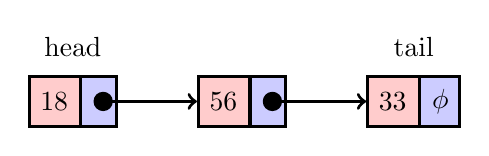
\begin{tikzpicture}[
      ->, start chain, very thick
    ]

      \node[list,on chain] (A) {18};
      \node[list,on chain] (B) {56};
      \node[list,on chain] (C) {33\nodepart{two}$\phi$};
      \draw[*->] let \p1 = (A.two), \p2 = (A.center) in (\x1,\y2) -- (B);
      \draw[*->] let \p1 = (B.two), \p2 = (B.center) in (\x1,\y2) -- (C);
      \node (head_text)[above=0.1cm of A]{head};
      \node (tail_text)[above=0.1cm of C]{tail};
    \end{tikzpicture}
    \caption{A singly-linked list.}
    \label{fig:singlelinkedlist}
  \end{figure}

  The $\phi$ symbol in the blue section of the tail node represents a null or empty pointer or reference, depending on the implementation language, that indicates the terminating node.

  Some implementations use a pointer or reference to a \emph{dummy} node that indicates the terminating node. The dummy node is not a true node in the linked list as it contains no data---it is simply a placeholder. Such a linked list might look like figure~\ref{fig:singlelinkedlist-dummy}.
  \begin{figure}[h]
    \centering
    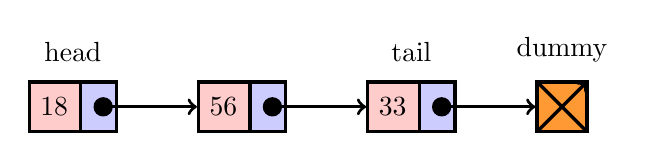
\begin{tikzpicture}[
      ->, start chain, very thick
    ]

      \node[list,on chain] (A) {18};
      \node[list,on chain] (B) {56};
      \node[list,on chain] (C) {33};
      \node[dummy]   (D) [right=of C] {};
      \node (head_text)[above=0.1cm of A]{head};
      \node (tail_text)[above=0.1cm of C]{tail};
      \node (dummy_text)[above=0.1cm of D]{dummy};
      \draw[*->] let \p1 = (A.two), \p2 = (A.center) in (\x1,\y2) -- (B);
      \draw[*->] let \p1 = (B.two), \p2 = (B.center) in (\x1,\y2) -- (C);
      \draw[*->] let \p1 = (C.two), \p2 = (C.center) in (\x1,\y2) -- (D);
    \end{tikzpicture}
    \caption{A singly-linked list with a dummy node.}
    \label{fig:singlelinkedlist-dummy}
  \end{figure}

  \subsection{Traversing a singly-linked list}
  Iterating accross a singly linked list is a bit more involved than simply using an index to reach an element in an array but the mechanism is still quite simple. Start at the head node, follow the pointer to the next node, and repeat until reaching the tail node, which is identified by its \emph{next} pointer being~$\phi$. The algorithm is shown in figure~\ref{fig:alg:singlelinkedlist-traverse}.
  \begin{figure}[h]
  \begin{algorithm}
    begin
      currentnode $\gets$ headnode
      while currentnode.next $\ne$ $\phi$:
        currentnode $\gets$ currentnode.next
    end\end{algorithm}
    \caption{Algorithm for traversing a singly-linked list.}
    \label{fig:alg:singlelinkedlist-traverse}
  \end{figure}

  To locate a specific node, while iterating over the list compare the data portion of the node to the target data value.
  \subsection{Adding nodes}
  Linked lists do not have a fixed length. They may grow or shrink to whatever size is needed, constrained only by available memory. There are procedures for appending nodes to the end of the list, prepending nodes at the front of the list, and for inserting a new node into a list.
  \subsubsection{Inserting into a singly-linked list}
  Inserting a node into a singly-linked list requires a few steps, but is generally more efficient than inserting an element into an array. To insert an element into an array, each following element must be moved down a position to make room for the new element. This is not the case with a linked list since each node points to its next node, wherever it may be in memory. Thus, a new node is inserted simply by manipulating the pointers.

  When inserting a new node into a singly-linked list, because the nodes point in only one direction, the new node in usually inserted \emph{after} a specified node. To insert a new node before a given node would require traversing the linked list until finding the node that precedes the desired node and inserting after that node.

  The algorithm for inserting into a singly-linked list is presented in figure~\ref{fig:alg:singlelinkedlist-insert}.
  \begin{figure}[h]
    \begin{algorithm}
      procedure insert(after_node, new_node)
      begin
        new_node.next $\gets$ after_node.next
        after_node.next $\gets$ new_node
      end\end{algorithm}
    \caption{Algorithm for inserting a node into a singly-linked list.}
    \label{fig:alg:singlelinkedlist-insert}
  \end{figure}

  Before applying the algorithm, a new node is created. This new node may reside anywhere in memory. The node's \emph{next} pointer does not yet have to point to anywhere of consequence and is often set to $\phi$. See figure~\ref{fig:singlelinkedlist-newnode}.
  \begin{figure}[h]
    \centering
    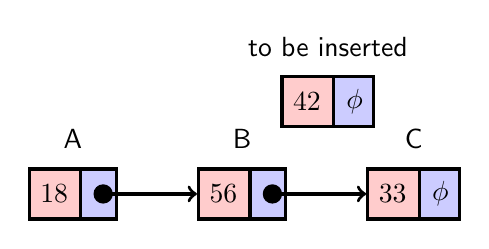
\begin{tikzpicture}[
      ->, start chain, very thick
    ]

      \node[list,on chain] (A) {18};
      \node[list,on chain] (B) {56};
      \node[list,on chain] (C) {33\nodepart{two}$\phi$};
      \node[list] (D) [above=.5cm of $(B.north)!0.5!(C.north)$] {42\nodepart{two}$\phi$};
      \node (a_label)[above=0.1cm of A]{\textsf{A}};
      \node (b_label)[above=0.1cm of B]{\textsf{B}};
      \node (c_label)[above=0.1cm of C]{\textsf{C}};
      \node (tbi_text)[above=0.1cm of D]{\textsf{to be inserted}};
      \draw[*->] let \p1 = (A.two), \p2 = (A.center) in (\x1,\y2) -- (B);
      \draw[*->] let \p1 = (B.two), \p2 = (B.center) in (\x1,\y2) -- (C);
    \end{tikzpicture}
    \caption{A new node to be inserted into a singly-linked list.}
    \label{fig:singlelinkedlist-newnode}
  \end{figure}

  Figures~\ref{fig:singlelinkedlist-insert-step-one} and \ref{fig:singlelinkedlist-insert-step-two} illustrate the process of inserting the new node into the linked list, between the second and third nodes, labeled~B and C respectively, in figure~\ref{fig:singlelinkedlist-newnode}. The list has been traversed and stopped at node B.

  Node B's \emph{next} pointer is copied into the new node's \emph{next} pointer, resulting in two nodes pointing to the same \emph{next} node, as shown in figure~\ref{fig:singlelinkedlist-insert-step-one}. This coresponds to line~3 in the insertion algorithm.
  \begin{figure}[H]
    \centering
    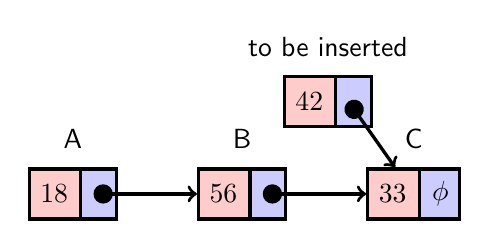
\begin{tikzpicture}[
      ->, start chain, very thick
    ]

      \node[list,on chain] (A) {18};
      \node[list,on chain] (B) {56};
      \node[list,on chain] (C) {33\nodepart{two}$\phi$};
      \node (a_label)[above=0.1cm of A]{\textsf{A}};
      \node (b_label)[above=0.1cm of B]{\textsf{B}};
      \node (c_label)[above=0.1cm of C]{\textsf{C}};
      \node[list] (D) [above=.5cm of $(B.north)!0.5!(C.north)$] {42};
      \node (tbi_text)[above=0.1cm of D]{\textsf{to be inserted}};
      \draw[*->] let \p1 = (A.two), \p2 = (A.center) in (\x1,\y2) -- (B);
      \draw[*->] let \p1 = (B.two), \p2 = (B.center) in (\x1,\y2) -- (C);
      \draw[*->] let \p1 = (D.two), \p2 = (D.center) in (\x1,\y2) -- (C);
    \end{tikzpicture}
    \caption{New node now points to its next node.}
    \label{fig:singlelinkedlist-insert-step-one}
  \end{figure}

  Node B's \emph{next} pointer is then set to the location of the new node, which is line~4 in the insertion algorithm. As seen in figure~\ref{fig:singlelinkedlist-insert-step-two}, the new node is fully inserted into the linked list.
  \begin{figure}[H]
    \centering
    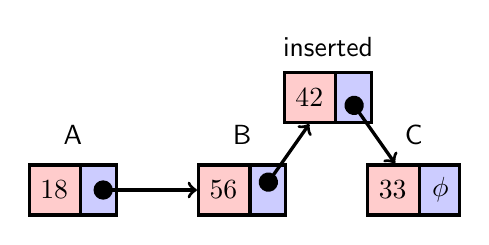
\begin{tikzpicture}[
      ->, start chain, very thick
    ]

      \node[list,on chain] (A) {18};
      \node[list,on chain] (B) {56};
      \node[list,on chain] (C) {33\nodepart{two}$\phi$};
      \node[list] (D) [above=.5cm of $(B.north)!0.5!(C.north)$] {42};
      \node (a_label)[above=0.1cm of A]{\textsf{A}};
      \node (b_label)[above=0.1cm of B]{\textsf{B}};
      \node (c_label)[above=0.1cm of C]{\textsf{C}};
      \node (tbi_text)[above=0.05cm of D]{\textsf{inserted}};
      \draw[*->] let \p1 = (A.two), \p2 = (A.center) in (\x1,\y2) -- (B);
      \draw[*->] let \p1 = (B.two), \p2 = (B.center) in (\x1,\y2) -- (D);
      \draw[*->] let \p1 = (D.two), \p2 = (D.center) in (\x1,\y2) -- (C);
    \end{tikzpicture}
    \caption{New node inserted, and previous node points to it.}
    \label{fig:singlelinkedlist-insert-step-two}
  \end{figure}

  Note that the new node was set to point at the next node \emph{before} setting the current node to point to the new node. Otherwise for a brief moment the new node is the last node in the list and the tail node is no longer part of the list. Additionally, if the new node's \emph{next} pointer was left unitialized on creation then that pointer may point anywhere, not at a valid list node. These issues are important in a multi-threaded environment. By having the new node point to the next node first, these problems are avoided.

  An unfortunate side effect of inserting a node after a specified node is that there is no node preceding the head node, making insertion of a node to be the new head node is problematic. Fortunately prepending a node to the front of a linked list is simple.

  \subsubsection{Prepending to the front of a singly-linked list}
  Adding a new node to the front of a linked list requires the current head node and the new node to be prepended. By setting the new node's \emph{next} pointer to the curent head node, the new node becomes the new head node.
  \begin{enumerate}
    \item Create the new node.
    \item Set the new node's \emph{next} pointer to point to the current head node.
    \item Set the head node to the new node
  \end{enumerate}
  The prepended node is now the new head node and the linked list is complete.

  \subsubsection{Appending to the end of a singly-linked list}
  Appending a new node to a linked list is simpler than inserting a node into the linked list, although the tail node must be located, which generally means either traversing the linked list or maintaining a pointer or reference to the tail node.
  \begin{enumerate}
    \item Create the new node and set its \emph{next} pointer to a null pointer or empty reference.
    \item Locate the tail node. If a large number of appends are expected, keeping a reference or pointer to the tail node can speed this process.
    \item Set the tail node's \emph{next} pointer to point to the new node.
  \end{enumerate}
  It is important to set the new node's next pointer to $\phi$ before changing the original tail node's pointer, to avoid having a brief time in which the new node is not a valid tail node.

  \subsection{Removing nodes}
  Removing a node from a singly-linked list is similar to the insertion process. Since there is no direct access to a node's previous node it is necessary to remove the node \emph{after} a given node.
  Figure~\ref{fig:singlelinkedlist-beforeremove} shows a singly-linked list with a node to be removed, node~C.
  \begin{figure}[H]
    \centering
    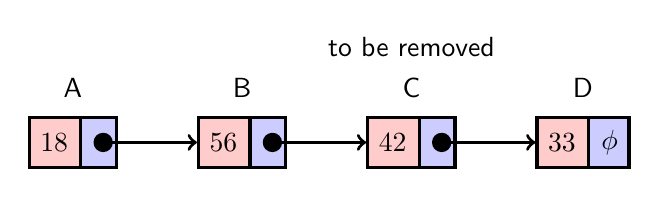
\begin{tikzpicture}[
      ->, start chain, very thick
    ]

      \node[list,on chain] (A) {18};
      \node[list,on chain] (B) {56};
      \node[list,on chain] (C) {42};
      \node[list,on chain] (D) {33\nodepart{two}$\phi$};
      \node (a_label)[above=0.1cm of A]{\textsf{A}};
      \node (b_label)[above=0.1cm of B]{\textsf{B}};
      \node (c_label)[above=0.1cm of C]{\textsf{C}};
      \node (d_label)[above=0.1cm of D]{\textsf{D}};
      %\node (tbr_text)[above=0.1cm of c_label]{\textsf{to be removed}};
      \node (tbr_text)[above=0pt of c_label]{\textsf{to be removed}};
      \draw[*->] let \p1 = (A.two), \p2 = (A.center) in (\x1,\y2) -- (B);
      \draw[*->] let \p1 = (B.two), \p2 = (B.center) in (\x1,\y2) -- (C);
      \draw[*->] let \p1 = (C.two), \p2 = (C.center) in (\x1,\y2) -- (D);
    \end{tikzpicture}
    \caption{A singly-linked list with a node to be removed.}
    \label{fig:singlelinkedlist-beforeremove}
  \end{figure}

  The following steps remove node~C by removing the node that comes after node~B in the linked list. Of course the first step is to locate node~B, which requires traversing the linked list until a node's next node is the one to be removed.

  Once node B, the node previous to the node to be removed, is found, the \emph{next} pointer from node C, the node to be removed, is copied to node B's \emph{next} pointer, resulting in the \emph{next} pointers for both nodes~A and B pointing to node D, as shown in figure~\ref{fig:singlelinkedlist-removelinkaround}.
  \begin{figure}[H]
    \centering
    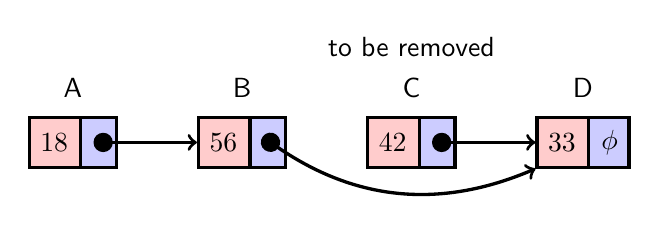
\begin{tikzpicture}[
      ->, start chain, very thick
    ]

      \node[list,on chain] (A) {18};
      \node[list,on chain] (B) {56};
      \node[list,on chain] (C) {42};
      \node[list,on chain] (D) {33\nodepart{two}$\phi$};
      \node (a_label)[above=0.1cm of A]{\textsf{A}};
      \node (b_label)[above=0.1cm of B]{\textsf{B}};
      \node (c_label)[above=0.1cm of C]{\textsf{C}};
      \node (d_label)[above=0.1cm of D]{\textsf{D}};
      \node (tbr_text)[above=0pt of c_label]{\textsf{to be removed}};
      \draw[*->] let \p1 = (A.two), \p2 = (A.center) in (\x1,\y2) -- (B);
      %\path[*->] let \p1 = (B.two), \p2 = (B.center) in (\x1,\y2) edge [bend right] (D);
      \path[*->] let \p1 = ($(B.two)+(0,0.175)$), \p2 = ($(B.center)+(0.0,0.075)$) in (\x1,\y2) edge [bend right] (D);
      \draw[*->] let \p1 = (C.two), \p2 = (C.center) in (\x1,\y2) -- (D);
    \end{tikzpicture}
    \caption{A singly-linked list with a Node B partially removed.}
    \label{fig:singlelinkedlist-removelinkaround}
  \end{figure}

  Finally, the \emph{next} pointer of the removed node is set to $\phi$, discarding that node's link and completing the removal, illustrated by figure~\ref{fig:singlelinkedlist-removed}
  \begin{figure}[H]
    \centering
    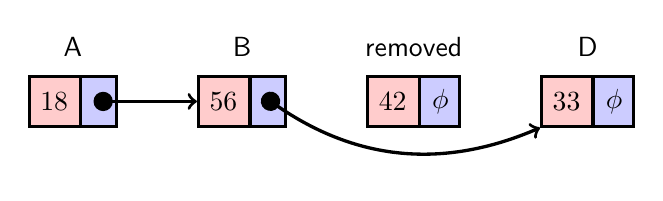
\begin{tikzpicture}[
      ->, start chain, very thick
    ]

      \node[list,on chain] (A) {18};
      \node[list,on chain] (B) {56};
      \node[list,on chain] (C) {42\nodepart{two}$\phi$};
      \node[list,on chain] (D) {33\nodepart{two}$\phi$};
      \node (b_label)[above=0.1cm of A]{\textsf{A}};
      \node (b_label)[above=0.1cm of B]{\textsf{B}};
      \node (d_label)[above=0.1cm of D]{\textsf{D}};
      \node (tbr_text)[above=0.1cm of C]{\textsf{removed}};
      \draw[*->] let \p1 = (A.two), \p2 = (A.center) in (\x1,\y2) -- (B);
      %\path[*->] let \p1 = (B.two), \p2 = (B.center) in (\x1,\y2) edge [bend right] (D);
      \path[*->] let \p1 = ($(B.two)+(0,0.175)$), \p2 = ($(B.center)+(0.0,0.075)$) in (\x1,\y2) edge [bend right] (D);
    \end{tikzpicture}
    \caption{A singly-linked list with Node C fully removed.}
    \label{fig:singlelinkedlist-removed}
  \end{figure}

  Removing the head node requires special handling since there is no node preceding it. Since most implementations maintain a reference to the head node, all that is required is that the maintained reference or pointer be set to the current head node's \emph{next} node. Then the former head node's \emph{next} pointer may be set to $\phi$ to completely disassociate that node from the linked list.

  The~C implementation of the singly-linked list in Part~\ref{part:implementation}, section~\ref{sect:C_implementation}, incorporates this logic into the \verb|sll_remove_node| function.

  \section{Doubly linked lists}
  A doubly-linked list is very similar to a singly-linked list. The primary difference is that a node contains a pointer to the previous node as well as a pointer to the next node. This allows the linked list to be traversed both forward and backward, and makes it much simpler to reach a node's predecessor. Figure~\ref{fig:doublelinkedlist} illustrates a doubly-linked list.
  \begin{figure}[H]
    \centering
    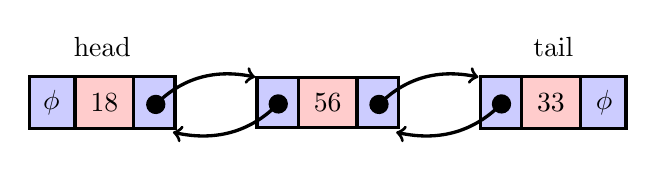
\begin{tikzpicture}[
      ->, start chain, very thick
    ]

      \node[dlist,on chain] (A) {\nodepart{one} $\phi$\nodepart{two} 18};
      \node[dlist,on chain] (B) {\nodepart{two} 56};
      \node[dlist,on chain] (C) {\nodepart{two} 33\nodepart{three}$\phi$};
      \node (head_text)[above=0.1cm of A]{head};
      \node (tail_text)[above=0.1cm of C]{tail};

      \path[*->] let \p1 = (A.three), \p2 = (A.two) in (\x1,\y2) edge [bend left] ($(B.one)+(-0.2,0.4)$);
      \path[*->] let \p1 = (B.three), \p2 = (B.two) in (\x1,\y2) edge [bend left] ($(C.one)+(-0.2,0.4)$);

      \path[*->] ($(B.one)+(0.175,0.15)$) edge [bend left] ($(A.three)+(0.3,-0.3)$);
      \path[*->] ($(C.one)+(0.175,0.15)$) edge [bend left] ($(B.three)+(0.3,-0.3)$);
    \end{tikzpicture}
    \caption{A doubly-linked list.}
    \label{fig:doublelinkedlist}
  \end{figure}
  % TODO: Write more about doubly-linked lists!!!

%  As with a singly-linked list, some implementations use pointers or references to \emph{dummy} nodes, one at either end of the linked list. The dummy nodes are not true nodes in the linked list as they contain no data---each is simply a placeholder. A doubly-linked list using dummy nodes might look like figure~\ref{fig:doublelinkedlist-dummy}.
%  \begin{figure}[h]
%    \centering
%    \begin{tikzpicture}[
%      ->, start chain, very thick
%    ]
%
%      \node[dummy,on chain] (D1) {};
%      \node[dlist,on chain] (A) {\nodepart{one} $\phi$\nodepart{two} 18};
%      \node[dlist,on chain] (B) {\nodepart{two} 56};
%      \node[dlist,on chain] (C) {\nodepart{two} 33\nodepart{three}$\phi$};
%      \node[dummy,on chain] (D2) {};
%      \node (dummy1_text)[above=0.1cm of D1]{dummy};
%      \node (head_text)[above=0.1cm of A]{head};
%      \node (tail_text)[above=0.1cm of C]{tail};
%      \node (dummy2_text)[above=0.1cm of D2]{dummy};
%      \draw[->] let \p1 = (D1), \p2 = (D1) in (\x1,\y2) -- (A);
%      \path[*->] let \p1 = (A.three), \p2 = (A.two) in (\x1,\y2) edge [bend left] ($(B.one)+(-0.2,0.4)$);
%      \path[*->] let \p1 = (B.three), \p2 = (B.two) in (\x1,\y2) edge [bend left] ($(C.one)+(-0.2,0.4)$);

%      \path[*->] ($(B.one)+(0.175,0.15)$) edge [bend left] ($(A.three)+(0.3,-0.3)$);
%      \path[*->] ($(C.one)+(0.175,0.15)$) edge [bend left] ($(B.three)+(0.3,-0.3)$);
%      \draw[*->] let \p1 = (C.three), \p2 = (C.center) in (\x1,\y2) -- (D2);
%    \end{tikzpicture}
%    \caption{A doubly-linked list with dummy nodes at the start and end.}
%    \label{fig:doublelinkedlist-dummy}
%  \end{figure}

  \subsection{Traversing a doubly-linked list}
  Traversing a doubly-linked list is exactly the same as with a singly-list list: follow each node's next pointer until the node that has no next pointer. One advantage of a doubly-linked list is that it can be traversed backward as well as forward. Follow each node's previous-node pointer until reaching the head node which has no previous-node pointer.
  \subsection{Adding nodes}
  Like singly-linked lists, doubly-linked lists do not have a fixed length and may grow or shrink to whatever size is needed, constrained only by available memory. New nodes may be easily appended to the end, prepended to the beginning, or inserted anywhere inside the linked list.
  \subsubsection{Inserting into a doubly-linked list}
  Inserting a node into a doubly-linked list involves essentially the same steps as used when inserting into a singly-linked list, but there are additional node pointers to contend with. However, an advantage to the additional nodes is that inserting a node before a given node is as efficient as inserting after a node.

  First a new node is created, which may be created anywhere in memory. The node's previous and next pointers are usually initialized to $\phi$. Figure~\ref{fig:doublelinkedlist-newnode} illustrates this.
  \begin{figure}[H]
    \centering
    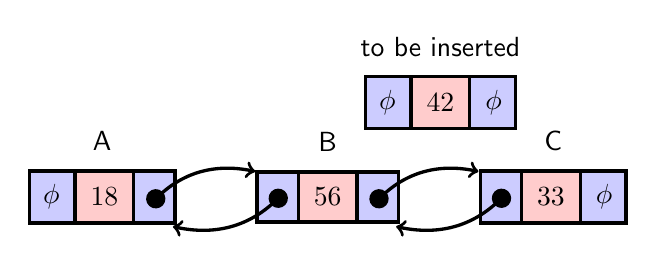
\begin{tikzpicture}[
      ->, start chain, very thick
    ]

      \node[dlist,on chain] (A) {\nodepart{one} $\phi$\nodepart{two} 18};
      \node[dlist,on chain] (B) {\nodepart{two} 56};
      \node[dlist,on chain] (C) {\nodepart{two} 33\nodepart{three}$\phi$};
      \node[dlist] (D) [above=.5cm of $(B.north)!0.5!(C.north)$] {\nodepart{one} $\phi$\nodepart{two}42\nodepart{three}$\phi$};
      \node (a_label)[above=0.1cm of A]{\textsf{A}};
      \node (b_label)[above=0.1cm of B]{\textsf{B}};
      \node (c_label)[above=0.1cm of C]{\textsf{C}};
      \node (tbi_text)[above=0.1cm of D]{\textsf{to be inserted}};

      \path[*->] let \p1 = (A.three), \p2 = (A.two) in (\x1,\y2) edge [bend left] ($(B.one)+(-0.2,0.4)$);
      \path[*->] let \p1 = (B.three), \p2 = (B.two) in (\x1,\y2) edge [bend left] ($(C.one)+(-0.2,0.4)$);

      \path[*->] ($(B.one)+(0.175,0.15)$) edge [bend left] ($(A.three)+(0.3,-0.3)$);
      \path[*->] ($(C.one)+(0.175,0.15)$) edge [bend left] ($(B.three)+(0.3,-0.3)$);
    \end{tikzpicture}
    \caption{A new node to be inserted into a doubly-linked list.}
    \label{fig:doublelinkedlist-newnode}
  \end{figure}

  Figures~\ref{fig:doublelinkedlist-insert-step-two} and \ref{fig:doublelinkedlist-insert-step-three} demonstrate the process of inserting the new node between nodes~B and C. Since nodes~B and C point to each other, forward and backward, the process is the same whether inserting after node~B or before node~C.

  The new node's previous pointer is set to point to node~B, and its next pointer is set to point to node~C, as shown in figure~\ref{fig:doublelinkedlist-insert-step-two}. It makes no difference whether the previous pointer is set first or the next pointer, but the two steps together should be done before modifying the pointers of existing nodes in the linked list.
  \begin{figure}[H]
    \centering
    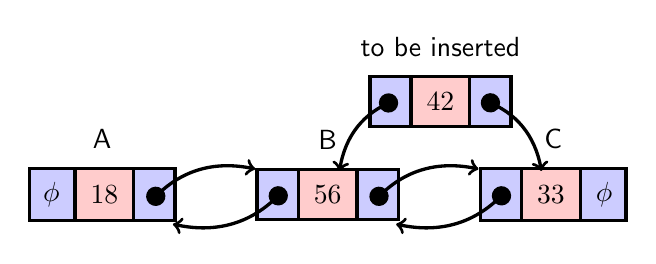
\begin{tikzpicture}[
      ->, start chain, very thick
    ]

      \node[dlist,on chain] (A) {\nodepart{one} $\phi$\nodepart{two} 18};
      \node[dlist,on chain] (B) {\nodepart{two} 56};
      \node[dlist,on chain] (C) {\nodepart{two} 33\nodepart{three}$\phi$};
      \node[dlist] (D) [above=.5cm of $(B.north)!0.5!(C.north)$] {\nodepart{two}42};
      \node (a_label)[above=0.1cm of A]{\textsf{A}};
      \node (b_label)[above=0.1cm of B]{\textsf{B}};
      \node (c_label)[above=0.1cm of C]{\textsf{C}};
      \node (tbi_text)[above=0.1cm of D]{\textsf{to be inserted}};

      \path[*->] let \p1 = (A.three), \p2 = (A.two) in (\x1,\y2) edge [bend left] ($(B.one)+(-0.2,0.4)$);
      \path[*->] let \p1 = (B.three), \p2 = (B.two) in (\x1,\y2) edge [bend left] ($(C.one)+(-0.2,0.4)$);

      \path[*->] ($(B.one)+(0.175,0.15)$) edge [bend left] ($(A.three)+(0.3,-0.3)$);
      \path[*->] ($(C.one)+(0.175,0.15)$) edge [bend left] ($(B.three)+(0.3,-0.3)$);
      \path[*->] ($(D.one)+(0.175,0.1)$) edge [bend right] ($(B)+(0.15,0.3)$);
      \path[*->] ($(D.three)+(-0.05,0.1)$) edge [bend left] ($(C)+(-0.15,0.3)$);
    \end{tikzpicture}
    \caption{New node now points to its previous and next nodes.}
    \label{fig:doublelinkedlist-insert-step-two}
  \end{figure}

  Once the new node's pointer have been set, node~B's \emph{next} pointer and node~C's \emph{previous} pointer are both set to the new node, as shown in figure~\ref{fig:doublelinkedlist-insert-step-three}, completing the insertion.
  \begin{figure}[H]
    \centering
    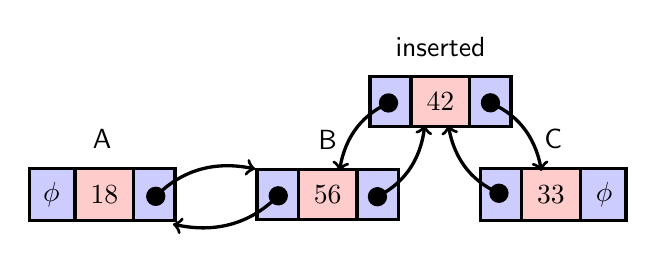
\begin{tikzpicture}[
      ->, start chain, very thick
    ]

      \node[dlist,on chain] (A) {\nodepart{one} $\phi$\nodepart{two} 18};
      \node[dlist,on chain] (B) {\nodepart{two} 56};
      \node[dlist,on chain] (C) {\nodepart{two} 33\nodepart{three}$\phi$};
      \node[dlist] (D) [above=.5cm of $(B.north)!0.5!(C.north)$] {\nodepart{two}42};
      \node (a_label)[above=0.1cm of A]{\textsf{A}};
      \node (b_label)[above=0.1cm of B]{\textsf{B}};
      \node (c_label)[above=0.1cm of C]{\textsf{C}};
      \node (tbi_text)[above=0.1cm of D]{\textsf{inserted}};

      \path[*->] let \p1 = (A.three), \p2 = (A.two) in (\x1,\y2) edge [bend left] ($(B.one)+(-0.2,0.4)$);
      \path[*->] ($(B.three)+(-0.05,0.0)$) edge [bend right] ($(D)+(-0.2,-0.3)$);

      \path[*->] ($(B.one)+(0.175,0.15)$) edge [bend left] ($(A.three)+(0.3,-0.3)$);
      \path[*->] ($(C.one)+(0.175,0.05)$) edge [bend left] ($(D)+(0.1,-0.3)$);
      \path[*->] ($(D.one)+(0.175,0.1)$) edge [bend right] ($(B)+(0.15,0.3)$);
      \path[*->] ($(D.three)+(-0.05,0.1)$) edge [bend left] ($(C)+(-0.15,0.3)$);
    \end{tikzpicture}
    \caption{New node inserted, both previous and next nodes point to it.}
    \label{fig:doublelinkedlist-insert-step-three}
  \end{figure}

  \subsubsection{Appending to the end of a doubly-linked list}
  Appending a node to the end of a doubly-linked list is similar to appending to a singly-linked list, with the exception of handling an additional node pointer.
  \begin{itemize}
    \item Create the new node and set its \emph{next} pointer to a null pointer or empty reference.
    \item Locate the tail node.
    \item Set the new node's \emph{previous} pointer to point to the current tail node.
    \item Set the current tail node's \emph{next} pointer to point to the new node.
  \end{itemize}
  As with a singly-linked list, the tail node must be located. Some implementations maintain a pointer or reference to the tail node for this purpose.

  \subsubsection{Prepending to the front of a doubly-linked list}
  Adding a new node to the beginning of a doubly-linked list is again similar to doing so to a singly-linked list. As with appending, there is another node pointer to consider.
  \begin{itemize}
    \item Create the new node, setting its \emph{previous} pointer to $\phi$.
    \item Set the new node's \emph{next} pointer to point to the current head node.
    \item Set the current head node's \emph{previous} pointer to the new node.
    \item Set the new head node to be the new node.
  \end{itemize}

  \subsection{Removing nodes}
  One advantage of a doubly-linked list over a singly-linked list is that a node can be removed directly, without the need to traverse the linked list looking for the previous node. Figure~\ref{fig:doublelinkedlist-before-remove} is a doubly-linked list before removing node~C.
  \begin{figure}[H]
    \centering
    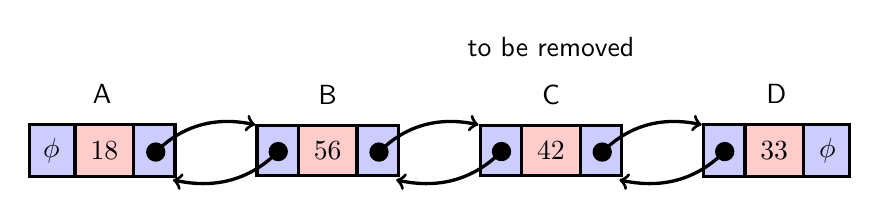
\begin{tikzpicture}[
      ->, start chain, very thick
    ]

    \node[dlist,on chain] (A) {\nodepart{one} $\phi$\nodepart{two} 18};
    \node[dlist,on chain] (B) {\nodepart{two} 56};
    \node[dlist,on chain] (C) {\nodepart{two} 42};
    \node[dlist,on chain] (D) {\nodepart{two} 33\nodepart{three}$\phi$};
    \node (a_label)[above=0.1cm of A]{\textsf{A}};
    \node (b_label)[above=0.1cm of B]{\textsf{B}};
    \node (c_label)[above=0.1cm of C]{\textsf{C}};
    \node (d_label)[above=0.1cm of D]{\textsf{D}};
    \node (tbr_label)[above=0.1cm of c_label]{\textsf{to be removed}};

    \path[*->] let \p1 = (A.three), \p2 = (A.two) in (\x1,\y2) edge [bend left] ($(B.one)+(-0.2,0.4)$);
    \path[*->] let \p1 = (B.three), \p2 = (B.two) in (\x1,\y2) edge [bend left] ($(C.one)+(-0.2,0.4)$);
    \path[*->] let \p1 = (C.three), \p2 = (C.two) in (\x1,\y2) edge [bend left] ($(D.one)+(-0.2,0.4)$);

    \path[*->] ($(B.one)+(0.175,0.15)$) edge [bend left] ($(A.three)+(0.3,-0.3)$);
    \path[*->] ($(C.one)+(0.175,0.15)$) edge [bend left] ($(B.three)+(0.3,-0.3)$);
    \path[*->] ($(D.one)+(0.175,0.15)$) edge [bend left] ($(C.three)+(0.3,-0.3)$);
  \end{tikzpicture}
    \caption{Doubly-linked list, node C to be removed.}
    \label{fig:doublelinkedlist-before-remove}
  \end{figure}

  First, node~C's \emph{previous} and \emph{next} pointers are used to locate the nodes prior to and following it. Node~B's \emph{next} pointer is set to point to node~D, and node~D's \emph{previous} pointer is set to point to node~B, as shown in figure~\ref{fig:doublelinkedlist-removing}.
  \begin{figure}[H]
    \centering
    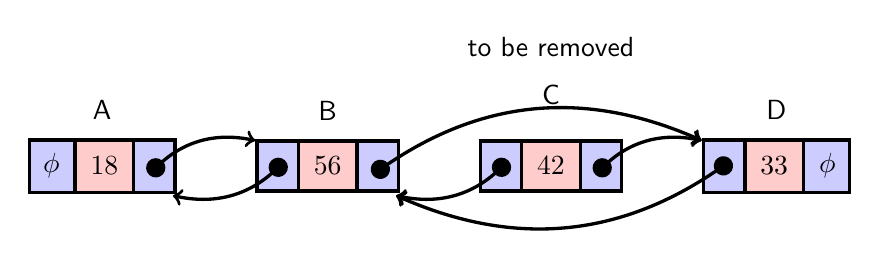
\begin{tikzpicture}[
      ->, start chain, very thick
    ]

    \node[dlist,on chain] (A) {\nodepart{one} $\phi$\nodepart{two} 18};
    \node[dlist,on chain] (B) {\nodepart{two} 56};
    \node[dlist,on chain] (C) {\nodepart{two} 42};
    \node[dlist,on chain] (D) {\nodepart{two} 33\nodepart{three}$\phi$};
    \node (a_label)[above=0.1cm of A]{\textsf{A}};
    \node (b_label)[above=0.1cm of B]{\textsf{B}};
    \node (c_label)[above=0.3cm of C]{\textsf{C}};
    \node (d_label)[above=0.1cm of D]{\textsf{D}};
    \node (tbr_label)[above=0.1cm of c_label]{\textsf{to be removed}};

    \path[*->] let \p1 = (A.three), \p2 = (A.two) in (\x1,\y2) edge [bend left] ($(B.one)+(-0.2,0.4)$);
    \path[*->] let \p1 = (B.three), \p2 = (B.two) in (\x1,\y2) edge [bend left] ($(D.one)+(-0.2,0.4)$);
    \path[*->] let \p1 = (C.three), \p2 = (C.two) in (\x1,\y2) edge [bend left] ($(D.one)+(-0.2,0.4)$);

    \path[*->] ($(B.one)+(0.175,0.15)$) edge [bend left] ($(A.three)+(0.3,-0.3)$);
    \path[*->] ($(C.one)+(0.175,0.15)$) edge [bend left] ($(B.three)+(0.3,-0.3)$);
    \path[*->] ($(D.one)+(0.175,0.15)$) edge [bend left] ($(B.three)+(0.3,-0.3)$);
  \end{tikzpicture}
    \caption{Nodes \textsf{B} and \textsf{D} now point to each other.}
    \label{fig:doublelinkedlist-removing}
  \end{figure}

  Once nodes B and C point to each other, node~C has effectively been removed. To ensure the removed node no longer refers to any node still in the linked list, its \emph{previous} and \emph{next} pointer are set to $\phi$, as illustrated in figure~\ref{fig:doublelinkedlist-after-remove}.
  \begin{figure}[H]
    \centering
    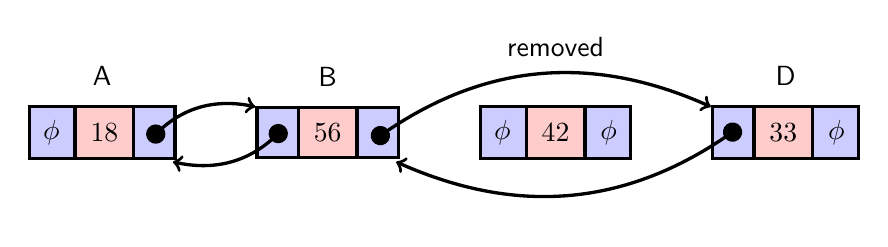
\begin{tikzpicture}[
      ->, start chain, very thick
    ]

    \node[dlist,on chain] (A) {\nodepart{one} $\phi$\nodepart{two} 18};
    \node[dlist,on chain] (B) {\nodepart{two} 56};
    \node[dlist,on chain] (C) {\nodepart{one}$\phi$\nodepart{two} 42\nodepart{three}$\phi$};
    \node[dlist,on chain] (D) {\nodepart{two} 33\nodepart{three}$\phi$};
    \node (a_label)[above=0.1cm of A]{\textsf{A}};
    \node (b_label)[above=0.1cm of B]{\textsf{B}};
    \node (c_label)[above=0.1cm of C]{\ };
    \node (d_label)[above=0.1cm of D]{\textsf{D}};
    \node (tbr_label)[above=0.1cm of c_label]{\textsf{removed}};

    \path[*->] let \p1 = (A.three), \p2 = (A.two) in (\x1,\y2) edge [bend left] ($(B.one)+(-0.2,0.4)$);
    \path[*->] let \p1 = (B.three), \p2 = (B.two) in (\x1,\y2) edge [bend left] ($(D.one)+(-0.2,0.4)$);

    \path[*->] ($(B.one)+(0.175,0.15)$) edge [bend left] ($(A.three)+(0.3,-0.3)$);
    \path[*->] ($(D.one)+(0.175,0.15)$) edge [bend left] ($(B.three)+(0.3,-0.3)$);
  \end{tikzpicture}
    \caption{Node C fully removed.}
    \label{fig:doublelinkedlist-after-remove}
  \end{figure}

  If the node to be removed is the head or tail node, the implementation must take care to not attempt to have a non-existant node point somewhere.

  \part{Implementation}\label{part:implementation}
  This part provides sample implementations of linked lists, in both the C and \Cpp\ languages. The C program implements a singly-linked list, and is simple and straightforward, while the \Cpp\ implementation utilizes an Object Oriented Programming approach to create a doubly-linked list.
  \section{C Implementation}
  \label{sect:C_implementation}
  Here we present an implementation of a singly-linked list in the C language. This implementation uses simple integers for the type of data stored in a node. The code can be easily modified to work with any data type.

  The implementation consists of two C source files, \verb|single_linked_list.h| and \verb|single_linked_list.c|.
  It begins in \verb|single_linked_list.h| by defining the linked list node type.
  \begin{lstc}[firstnumber=1]
typedef struct _sll_node
{
  int data;
  struct _sll_node *next;
} sll_node;\end{lstc}
  Following node type definition are prototypes for the functions operating on the linked list.
  \begin{lstc}
sll_node *sll_create_node(int data);
sll_node *sll_find_data(sll_node *start, int data);
sll_node *sll_find_tail_node(sll_node *start);
sll_node *sll_append_node(sll_node **head, sll_node *node);
sll_node *sll_append_data(sll_node **head, int data);
sll_node *sll_insert_node_after(sll_node *after, sll_node *node);
sll_node *sll_insert_data_after(sll_node *after, int data);
sll_node *sll_prepend_node(sll_node **head, sll_node *node);
sll_node *sll_prepend_data(sll_node **head, int data);
sll_node *sll_remove_after(sll_node **head, sll_node *node);
sll_node *sll_remove_node(sll_node **head, sll_node *node);
void sll_erase(sll_node **head);\end{lstc}
  Many of these functions take the head node as a pointer-to-pointer to the \verb|ssl_node| structure. This is because these operations have at least the potential to modify the linked list such that there would be a new head node and it is necessary to keep track of the current head node.

  This completes \verb|single_linked_list.h|. The function implementations are in \verb|single_linked_list.c|.

  The first thing to do is to \verb|#include| the C library's \verb|stdlib.h| file and the \verb|single_linked_list.h| file defined above. The \verb|stdlib.h| file contains declarations for the functions \verb|malloc| and \verb|free| which will be used to allocate and deallocate memory for the linked list nodes.
  \begin{lstc}[firstnumber=1]
#include <stdlib.h>
#include "single_linked_list.h"\end{lstc}
  Next is the implementation code for the functions that operate on the linked list, starting with \verb|sll_create_node|.
  \begin{lstc}
sll_node *sll_create_node(int data) {
  sll_node *node = (sll_node *)malloc(sizeof(sll_node));
  if (node != NULL) {
    node->next = NULL;
    node->data = data;
  }

  return node;
}\end{lstc}
  On line 4 memory is allocated for the new node using the C library's \verb|malloc| function. Line 5 tests that the allocation was successful, then lines 6 and 7 set the node's \verb|next| pointer to \verb|NULL| and copies the data into the node. Setting the node's \verb|next| pointer to \verb|NULL| is not strictly required, but doing so is a safety measure against a possible runaway list. Finally, on line 10, the function returns a pointer to the newly created node.

  Next is the definition of the \verb|sll_find_data| function which traverses the list, begining at the head node, looking for the specified data and returning a pointer to the node containing that data, or \verb|NULL| if the data was not found.
  \begin{lstc}
sll_node *sll_find_data(sll_node *start, int data) {
  while (start != NULL) {
    if (start->data == data)
      break;
    start = start->next;
  }

  return start; // Will be NULL if data is not found
}\end{lstc}
  The \verb|while| statement on line 13 moves the \verb|start| pointer from node to node until either the data node is found or until \verb|start| contains the \verb|NULL| pointer value from the \verb|next| pointer of the tail node. Line 16 advances the \verb|start| pointer to the next node in the linked list.

  Next, the \verb|find_tail_node| function is defined. This function traverses the linked list starting at a specified node until the tail node is found. The starting node might usually be the head node, but that is not required.
  \begin{lstc}
sll_node *sll_find_tail_node(sll_node *start) {
  if (start != NULL)
    while (start->next != NULL)
      start = start->next;

  return start;
}\end{lstc}
  Line 22, tests the \verb|start| node to ensure that it is not \verb|NULL|. If the \verb|start| node is \verb|NULL|, control falls to the \verb|return| statment on line~26.

  Lines 23 and~24 use the \verb|start| parameter to traverse the list, updating \verb|start| to point to the next node in the linked list until the node's \verb|next| pointer is \verb|NULL|, indicating that the node is the tail node. Line~26 returns a pointer to that node.

  The \verb|sll_append_node| function appends a new node to the end of the list.
  \begin{lstc}
sll_node *sll_append_node(sll_node **head, sll_node *node) {
  if (*head == NULL)
    *head = node;
  else
    list_find_tail_node(*head)->next = node;

  return node;
}\end{lstc}
  The function parameter list on line 28 takes \verb|head| as a pointer-to-pointer to an \verb|ssl_node| structure. This allows the pointer to the head node to be modified if necessary. In this case, if the linked list is empty as indicated by the head pointer being \verb|NULL| (line~29) then the new node becomes the new head node on line~31.

  If the linked list is not empty, then line 32 locates the tail node and sets its \verb|next| pointer to point to the new node. A pointer to the new node is returned.

  The \verb|sll_append_data| function is very simple.
  \begin{lstc}
sll_node *sll_append_data(sll_node **head, int data) {
  return sll_append_node(head, sll_create_node(data));
}\end{lstc}
  A new node is created by calling \verb|sll_create_node| with the specified data, then that node is appended to the end of the linked list by calling \verb|sll_append_node|. A pointer to the newly created and appended node is returned. Again, the head of the linked list may be changed to point to a new node.

  \verb|sll_insert_node_after| inserts a new node immediately following a given existing node.
  \begin{lstc}
sll_node *sll_insert_node_after(sll_node *after, sll_node *node) {
  node->next = after->next;
  after->next = node;

  return node;
}\end{lstc}
  On line 40 the new node's \verb|next| pointer is set to \verb|after|'s \verb|next| pointer. There are now two nodes pointing to the same following node. Then, on line~41, the \verb|next| pointer of the \verb|after| node is modified to point to the new node, completing the link. These are the steps illustrated in figures~\ref{fig:singlelinkedlist-insert-step-one} and~\ref{fig:singlelinkedlist-insert-step-two} in Part~\ref{part:description}.

  The \verb|sll_insert_data_after| function is similar to the \verb|sll_append_data| function. It calls \verb|sll_create_node| to create a new node, then passes that node pointer on to \verb|sll_insert_node_after| and returns a pointer to the new node.
  \begin{lstc}
sll_node *sll_insert_data_after(sll_node *after, int data) {
  return sll_insert_node_after(after, sll_create_node(data));
}\end{lstc}

  The \verb|sll_prepend_node| function adds a new node to the front of the linked list, making that node the new head node.
  \begin{lstc}
sll_node *prepend_node(sll_node **head, sll_node *node) {
  node->next = *head;
  *head = node;

  return node;
}\end{lstc}
  Line 49 sets the new node's \verb|next| pointer to point to the current head node.

  Line 50 directly changes the head node by setting \verb|*head| to the new node pointer. Again, note the additional level of indirection. \verb|node| is now the new head node of the linked list.

  The \verb|sll_prepend_data| function calls \verb|sll_create_node| and \verb|sll_prepend_node| to create a new node with the specified data and make that node the new head of the linked list.
  \begin{lstc}
sll_node *sll_prepend_data(sll_node **head, int data) {
  return sll_prepend_node(head, sll_create_node(data));
}\end{lstc}

  The implementation provides two functions for removing a linked list node. The first, \verb|sll_remove_node_after| removes the node \emph{following} the given node.
  \begin{lstc}
sll_node *sll_remove_node_after(sll_node **head, sll_node *node) {
  if (node->next != NULL) {
    sll_node *next = node->next;

    node->next = next->next;
    free(next);
  }

  return node->next;
}\end{lstc}
  Line~58 determines whether the passed-in node has a node following it. If so, that node will be removed and line~59 saves a pointer to that node. Line~61 sets the passed-in node's next pointer to point to the node following the node to be removed. This unlinks the desired node from the linked list. That node's next pointer still points to the following node, but it is not necessary to reset that pointer since line~66 disposes of the removed node with the C~Library's \verb|free| function.

  Note that only the memory for each node is deallocated. If the \verb|data| portion of the node is a pointer or contains pointers to allocated memory, it is the user's responsibility to perform any required memory management before removing the node.

  Whether there was a next node to remove or not, on line~65 the function returns a pointer to the node now following the passed-in node, which might be \verb|NULL|.

  The \verb|sll_remove_node| function removes a node from a linked list, and is the longest of this implementation. If the node to be removed is the head node, the next node in the list must be made the new head node. Otherwise the list must be traversed to locate the node that appears before the one to be removed.
  \begin{lstc}
sll_node *sll_remove_node(sll_node **head, sll_node *node) {
  if (node == *head) {
    *head = node->next;
    free(node);
    return *head;
  }
  else {
    sll_node *previous = *head;

    while (previous != NULL) {
      if (previous->next == node)
        return sll_remove_node_after(head, node);

      previous = previous->next;
    }
  }

  return NULL;
}\end{lstc}
  Line~68 determines whether the node to be removed is the head node and if so line~69 resets the current head node to the next node, unlinking the node from the linked list. The removed node is then disposed of with the standard C library function \verb|free| and the new head node is returned.

  If the node to be removed is not the head node, the list must be traversed from the beginning to locate the node previous to the one being removed. A new variable is created to traverse the linked list on line~74, and is initialized to point to the head node. A \verb|while| loop is employed on line~83 to traverse the list until the \verb|previous| variable becomes NULL, in which case the node was not found.

  Inside the \verb|while| loop, on line~77, if \verb|previous|'s \verb|next| pointer points to the node to be removed then \verb|node|'s previous node has been found. That node is passed to the \verb|sll_remove_node_after| function to perform the actual removal, and the result of that function is returned.

  The final function in the C implementation is \verb|sll_erase|, which traverses the linked list, freeing the memory allocated for each node.
  \begin{lstc}
void sll_erase(sll_node **head) {
  sll_node *current = *head;

  while (current != NULL) {
    sll_node *next = current->next;

    free(current);
    current = next;
  }

  *head = NULL;
}\end{lstc}
  The function is passed a pointer-to-pointer to the head node because the head node will ultimately be set to \verb|NULL| to indicate that the linked list is empty.

  On line~87 a new node variable is created to point to the current node as the linked list is being traversed. Line~89 begins the \verb|while| loop that traverses the linked list. The \verb|current| node's \verb|next| pointer is stored in a temporary variable and the memory allocated to the \verb|current| node is deallocated by calling the C library's \verb|free| function, on line~92. \verb|current| is set to point to the next node in the linked list, the value stored in the temporary variable, and the loop continues until there are no more nodes in the list.

  Finally, the head node is set to NULL, indicating that the linked list is now empty.

  This completes the implementation of a singly-linked list in C, produced in under~100 lines of C code.

  Implementing a doubly-linked list in C is similar to a singly-linked list. The main difference in a doubly-linked list is that the node structure contains an additional pointer to point to the previous node, making it possible to traverse the linked list in both directions.

  A complete implementation of a doubly-linked list in C is available for download from the git repository.

  \section{\texorpdfstring{\Cpp}{C++} Implementation}
  \label{sect:Cpp_implementation}
  This section presents an implementation of a doubly-linked list in the \Cpp\ language. The implementation utilizes Object Oriented Programming principals, particularly encapsulation. Templates are also used so a linked list can use any copyable data type.

  This is a header-only implementation consisting only of \verb|DoubleLinkedList.h|. The user need only include the header file. No additional library or object code is required.

  The code produces a basic linked list. There are no exceptions thrown as there is no real error checking.

  The implementation begins by defining the \verb|DoubleLinkedList| class.
  \begin{lstcpp}[firstnumber=1]
template<typename T>
class DoubleLinkedList {\end{lstcpp}
  \verb|DoubleLinkedList| is a class template, allowing the linked list to be used with any copyable data type.

  The core of a linked list is the \emph{node}. In this implementation, the node is defined as a nested, public class type.
  \begin{lstcpp}
public:
  class node_t {
  private:
    T       _data;
    node_t *_next{nullptr};
    node_t *_prev{nullptr};

  public:
    explicit node_t(const T &data)
      : _data{data}
    {}

    node_t(const node_t &) = delete;
    node_t & operator=(const node_t &) = delete;\end{lstcpp}
  Line~3 begins the definition of the \verb|node_t| class which defines the linked list node. The \verb|node_t| class defines three private data members on lines 6, 7 and 8. The \verb|_data| member is of type \verb|T|, the declared template type, and holds the node's copy of the data stored in the linked list. The \verb|_next| and \verb|_prev| members, of type \verb|node_t *|, are pointers to the next and previous nodes, respectively, in the linked list. Lines 11--13 define the \verb|node_t| type's \verb|explicit| constructor, which takes a reference to an object of type \verb|T|. A node is not copyable and it is not assignable, as specified by lines~15 and 16.

  The \verb|node_t| class contains three public functions, \verb|data()|, \verb|next()|, and \verb|prev()| which provide access to the content of the linked list item data and read access to the node's \emph{next} and \emph{previous} pointers. The class also provides two private functions, \verb|next(const node_t *node)| and \verb|prev(const node_t *prev)|. These functions are private because they are meant to be called only by the \verb|DoubleLinkedList| class to set the values of the node's \emph{next} and \emph{prev} pointers.
  \begin{lstcpp}
    T &data() noexcept {
        return _data;
    }

    node_t *next() const noexcept {
        return _next;
    }

    node_t *prev() const noexcept {
        return _prev;
    }

  private:
    void next(node_t *node) {
      _next = node;
    }

    void prev(node_t *node) {
      _prev = node;
    }

    friend DoubleLinkedList;
  };\end{lstcpp}
  Finally, on line~38 the \verb|DoubleLinkedList| class is declared to be a \verb|friend| of the \verb|node_t| class. This allows \verb|DoubleLinkedList| access to the node's private functions and data members.

  That is the entire definition of the nested \verb|node_t| class. The definition of the \verb|DoubleLinkedList| class continues with the definition of three private data members.
  \begin{lstcpp}
private:
  node_t *_head_node{nullptr};
  node_t *_tail_node{nullptr};
  size_t  _count{0};\end{lstcpp}
  The \verb|DoubleLinkedList| class maintains the pointer to the head node so the user does not have to. To increase the speed of some operations, and as a convenience to the user, the class maintains a pointer to the tail node, and a count of the number of nodes currently in the linked list.

  The implementation of the \verb|DoubleLinkedList| class continues, beginning with construction and destruction.
  \begin{lstcpp}
public:
  DoubleLinkedList() noexcept = default;

  DoubleLinkedList(const DoubleLinkedList &) = delete;
  DoubleLinkedList & operator=(const DoubleLinkedList &) = delete;

  ~DoubleLinkedList() {
    erase();
  }\end{lstcpp}
  The default constructor is not required to perform any specific initialization, so it is declared as \verb|default| on line~45 to have the compiler generate it. The class is not copyable and not assignable, so lines~47 and 48 use the \verb|delete| keyword to tell the compiler to not generate those functions.

  The destructor, on line~50, is implemented because it must delete all of the linked list's nodes. The \verb|erase| function, which is defined later, performs this task.

  Following the constructors and destructor are the operational functions of \verb|DoubleLinkedList|, beginning with the \verb|head|, \verb|tail|, \verb|size|, and \verb|is_empty| functions.

%  \begin{minipage}{\textwidth}
  \begin{lstcpp}
  node *head() const noexcept {
    return _head_node;
  }

  node_t *tail() const noexcept {
    return _tail_node;
  }

  size_t size() const noexcept {
    return _count;
  }

  bool is_empty() const noexcept {
    return head() == nullptr;
  }\end{lstcpp}
%  \end{minipage}
  The \verb|head| function simply returns the \verb|_head_node| member. On line~57 the \verb|tail| function returns the \verb|_tail_node| data member. The \verb|size| function returns the \verb|_count| member and the \verb|is_empty| function returns a \verb|bool| indicating whether the \verb|_head_node| is equal to \verb|nullptr|.

  Next are the functions that add and remove items from the linked list.
  The first is the \verb|prepend| function, which adds an item to the front of the linked list, before the current head node. The added item becomes the new head node.
  \begin{lstcpp}
  node_t *prepend(const T &data) {
    node_t *new_node{new node_t(data)};

    new_node->next(head());
    if (is_empty())
        _tail_node = new_node;
    else
        head()->prev(new_node);
    _head_node = new_node;

    ++_count;

    return new_node;
  }\end{lstcpp}
  The \verb|prepend| function takes a \verb|const| reference to an object of type \verb|T|, which is the type given to the class' template parameter. On line~69 a new node is allocated and constructed using the \verb|new| operator. The new node's \emph{next} pointer is then set to point to the current head node, which may or may not be \verb|nullptr|. If the linked list is empty, line~73 sets the \verb|_tail_node| member to the new node since the new node will be the only node in the list. Otherwise there is a head node and its \emph{prev} node is set to the new node on line~75. In either case, line~76 sets the current head node to be the new node. The count is incremented and the pointer to the new node is returned.

  Note that this function invokes the node's private \verb|next(node_t *node)| and \verb|prev(node_t *node)| member functions. This is possible because the \verb|node_t| class declared \verb|DoubleLinkedList| to be a \verb|friend|.

  The next function to be defined is \verb|insert_after|, which inserts a new item into the linked list immediately following a given node.
  \begin{lstcpp}
  node_t *insert_after(const T &data, node_t *node) {
    node_t *new_node{new node_t(data)};

    new_node->_next = node->_next;
    new_node->_prev = node;
    node->_next = new_node;
    if (new_node->_next == nullptr)
      _tail_node = new_node;
    else
      new_node->_next->_prev = new_node;

    ++_count;

    return new_node;
  }\end{lstcpp}
  \verb|insert_after| takes two parameters, a \verb|const| reference to the data to be inserted and a pointer to a node after which the new data will be inserted.

  On line~83 a new node is allocated and constructed. Lines 85--87 stitch the nodes together into the linked list by setting the new node's \verb|_next| pointer to the passed-in node's \verb|_next| pointer, setting the new node's \verb|_prev| pointer to the passed in node, then finally setting the passed-in node's \verb|_next| pointer to point to the new node, completing the insertion. These are the steps illustrated in figures~\ref{fig:doublelinkedlist-insert-step-two} and \ref{fig:doublelinkedlist-insert-step-three} in Part~\ref{part:description}. If the new node has no next pointer then it is the new tail node as well, and line~89 sets the linked list's tail node to be the new node. Otherwise the new node is being inserted not only after the specified node, but also before the following node, so the following node's \emph{prev} pointer is set to the new node on line~91. The node count is incremented and a pointer to the new node is returned.

  A doubly-linked list provides the ability to easily insert a new element before a given node, something that is more involved with a singly-linked list.
  \begin{lstcpp}
  node_t *insert_before(const T &data, node_t *node) {
    return node == head() ? prepend(data)
                          : insert_after(data, node->prev());
  }\end{lstcpp}
  The \verb|insert_before| function tests whether the specified node is the head node. If true, the new node is prepended to the front of the linked list and becomes the new head node. Otherwise, there is a node preceding the specified node and \verb|insert_after| is called with that preceding node.

  The \verb|append| function adds a new item to the end of the linked list, following the tail node.
  \begin{lstcpp}
  node_t *append(const T &data) {
    return is_empty() ? prepend(data)
                      : insert_after(data, tail());
  }\end{lstcpp}
  Again, the \verb|append| function takes a \verb|const| reference to an object of type \verb|T|. If the linked list is empty then the data object is passed on to the \verb|prepend| function defined above. Otherwise the data is given to the \verb|insert_after| function to be inserted after the tail node.

  A doubly-linked list provides for a relatively simple mechanism for removing a node directly, eliminating the need for a \verb|remove_after| function. The \verb|remove| function takes as a parameter the node to be removed, and returns a pointer to the following node if any.
  \begin{lstcpp}
  node_t *remove(node_t *node) {
    node_t *next_node{node->next()};

    if (node == head()) {
      if (next_node == nullptr) {
        _head_node = _tail_node = nullptr;
      }
      else {
        next_node->prev(nullptr);
        _head_node = next_node;
      }
    }
    else if (node == tail()) {
      node->prev()->next(nullptr);
      _tail_node = node->prev();
    }
    else {
      node->prev()->next(next_node);
      next_node->prev(node->prev());
    }

    delete node;
    --_count;

    return next_node;
  }\end{lstcpp}

  On line~106 a pointer to the specified node's \emph{next} node is stored.

  Line~108 determines if the node to be removed is the head node. If so, then if the head node is the only node in the linked list (line~109) then the head and tail nodes are set to \verb|nullptr| making the linked list empty. Otherwise, there is a next node and that node's \emph{prev} pointer is set to \verb|nullptr|, making it the new head node.

  If the node to be removed is not the head node but is instead the tail node (line~117), then the node prior to the specified node is made the new tail node.

  If the node to be removed is neither the head nor tail node (the \verb|else| on line~121), the node is extricated from the linked list by adjusting the \emph{next} pointer of the previous node and the \emph{next} pointer on the next node.

  Finally, the memory for the node to be removed is reclaimed, the node count is decremented, and the following node is returned. That node might be \verb|nullptr|.

  Next is the \verb|erase| function, which was used in the destructor to remove all nodes in the linked list. It is a public member function so it is available for users of the class as well.
  \begin{lstcpp}
  void erase() {
    node_t *current{head()};

    while (current != nullptr) {
      node_t *next{current->next()};

      delete current;
      current = next;
    }

    _head_node = _tail_node = nullptr;
    _count = 0;
  }\end{lstcpp}
  The \verb|erase| function iterates all nodes in the list, beginning with the head node on line~132. The \verb|while| statement line~134 loops until the current node is \verb|nullptr|, indicating the end of the linked list. For each node in the linked list, lines 135--138 save the value of the current node's \emph{next} pointer, free memory allocated to the node with the \verb|delete| operator, then re-assign the current node to the saved pointer to the next node. Once all nodes have been freed the head and tail nodes are set to \verb|nullptr| and the node counter is set to 0 signifying that the linked list is empty.

  One more function in the public interface remains. The \verb|find| function traverses the linked list and returns the first node that contains a specified data value.
  \begin{lstcpp}
  node_t *find(const T &data) {
    node_t *current{head()};

    while (current != nullptr) {
      if (current->data() == data)
        break;

      current = current->next();
    }

    return current;
  }\end{lstcpp}
  The search begins at the head node on line~145. While the current node pointer in the search points to an existing node (line~147), if the current node's data member is equal to the \verb|data| parameter the loop terminates (lines~148 and 149), otherwise the current node pointer is set to the next node in the linked list. Regardless of how the loop terminated, the current node is either the node containing the data or is \verb|nullptr|, indicating that the end of the linked list was reached without finding the data. On line~154 that node value is returned.


  This completes the implementation of a doubly-linked list in \Cpp, produced in~155 lines of code.

  Implementing a singly-linked list in \Cpp\ is similar to a doubly-linked list. The main difference in a singly-linked list is that the node structure contains only the node's data and a pointer to the next node, so it is possible to traverse such a linked in only in the forward direction.

  A complete implementation of a singly-linked list in \Cpp\ is available for download from the git repository.

\end{document}
